% ######################################
% ######### Masterdatei ################
% ######################################

\documentclass[    
	a4paper,          % Papierformat
    twoside,          % zweiseitiger Druck
    12pt,             % Schriftgröße
    halfparskip,      % eine halbe Zeile Abstand zw. Absätzen
    listof=totoc,
    ]{scrbook}
\usepackage[a4paper]{geometry}
\usepackage[utf8]{inputenc}
\usepackage[T1]{fontenc}
\usepackage{longtable}
\usepackage[ngerman]{babel}
\usepackage{lmodern}
\usepackage{amsmath}
\usepackage{mathtools}
\usepackage{amsfonts}
\usepackage{amssymb}
\usepackage{fancyhdr}
\usepackage{graphicx}
\usepackage{appendix}
\usepackage{setspace}
\usepackage{rotating}
\usepackage{longtable}
\usepackage{multicol}
\usepackage{enumitem}
\usepackage{url}
\usepackage{array}
\usepackage[usenames,dvipsnames]{color}
\usepackage{xcolor}
\usepackage{tikz}
\usepackage{listings}
\usepackage{caption}
\usepackage[section]{placeins}
\usepackage{blindtext}
\usepackage[numbers,square]{natbib}
\usepackage[section]{placeins}
\usepackage[pdftitle={Arbeitstitel}, % Titel
			pdfsubject={Arbeitsthema}, % Thema
			pdfauthor={Autor}, % Autor
			linkcolor=black, % Linkfarbe im PDF
			colorlinks=true, % Links einfärben?
			urlcolor=black, % URL-Farbe im PDF
			citecolor=black]{hyperref} % erscheint in Eigenschaften des Dokuments
\usepackage{nameref}
\makeatletter
\newcommand*{\currentname}{\@currentlabelname}
\makeatother

\setlength\parindent{0pt}
\onehalfspacing

% FÜr Quellcodebeispiele
\DeclareCaptionFont{white}{\color{white}}
\DeclareCaptionFormat{listing}{\colorbox{gray}{\parbox{\textwidth}{#1#2#3}}}
\captionsetup[lstlisting]{format=listing,labelfont=white,textfont=white}

%Um lange URLs in \url{} richtig umbrechen zu können
\def\UrlBreaks{\do\a\do\b\do\c\do\d\do\e\do\f\do\g\do\h\do\i\do\j\do\k\do\l \do\m\do\n\do\o\do\p\do\q\do\r\do\s\do\t\do\u\do\v\do\w\do\x\do\y\do\z\do\0 \do\1\do\2\do\3\do\4\do\5\do\6\do\7\do\8\do\9\do\-\do\_}
\urlstyle{same}  %Pakete und Definitionen

\begin{document}

% Definition Kopf und Fußzeile
\fancyhf{}
\renewcommand{\sectionmark}[1]{\markboth{#1}{}}
\renewcommand{\headrulewidth}{0.4pt}
\fancyhead[RE,OL]{{\nouppercase{\leftmark}}}
\fancyfoot[LE,OR]{\thepage}

% Vor dem Inhalt
\pagestyle{empty}
\frontmatter 
\begin{titlepage}
\begin{center}
\hrule
\vspace{0.5cm}
\Huge Titel der Arbeit
\vspace{0.5cm}
\hrule
\vspace{2.5cm}
\large Bachelorarbeit\\
\large zur Erlangung des akademischen Grades\\
\large Bachelor of Science (B. Sc.)\\
\large im Studiengang Informatik\\
\end{center}
\vfill
\begin{tabbing}
AbstandEinssssssss \= second \= third \kill
Verfasser: \> Micky Maus\\
Matrikelnummer: \> 314159265\\
Erstprüfer: \> Prof. Dr. Donald Duck\\
Zweitprüfer: \> Goofy\\
Hochschule: \> Entenhausener Hochschule\\
Unternehmen: \> Dagoberts Gewinnbring GmbH\\
Datum: \> \today
\end{tabbing}
\end{titlepage}


\definecolor{light-gray}{gray}{0.9}
\definecolor{pblue}{rgb}{0.13,0.13,1}
\definecolor{pgreen}{rgb}{0,0.5,0}
\definecolor{pred}{rgb}{0.9,0,0}
\definecolor{pgrey}{rgb}{0.46,0.45,0.48}
\definecolor{pgreen}{rgb}{0.50,2.05,0.50}
\definecolor{ppurple}{rgb}{0.50,0.205,0.50}

% Escape folgende Character
\lstset{literate=
	{á}{{\'a}}1 {é}{{\'e}}1 {í}{{\'i}}1 {ó}{{\'o}}1 {ú}{{\'u}}1
	{Á}{{\'A}}1 {É}{{\'E}}1 {Í}{{\'I}}1 {Ó}{{\'O}}1 {Ú}{{\'U}}1
	{à}{{\`a}}1 {è}{{\`e}}1 {ì}{{\`i}}1 {ò}{{\`o}}1 {ù}{{\`u}}1
	{À}{{\`A}}1 {È}{{\'E}}1 {Ì}{{\`I}}1 {Ò}{{\`O}}1 {Ù}{{\`U}}1
	{ä}{{\"a}}1 {ë}{{\"e}}1 {ï}{{\"i}}1 {ö}{{\"o}}1 {ü}{{\"u}}1
	{Ä}{{\"A}}1 {Ë}{{\"E}}1 {Ï}{{\"I}}1 {Ö}{{\"O}}1 {Ü}{{\"U}}1
	{â}{{\^a}}1 {ê}{{\^e}}1 {î}{{\^i}}1 {ô}{{\^o}}1 {û}{{\^u}}1
	{Â}{{\^A}}1 {Ê}{{\^E}}1 {Î}{{\^I}}1 {Ô}{{\^O}}1 {Û}{{\^U}}1
	{œ}{{\oe}}1 {Œ}{{\OE}}1 {æ}{{\ae}}1 {Æ}{{\AE}}1 {ß}{{\ss}}1
	{ç}{{\c c}}1 {Ç}{{\c C}}1 {ø}{{\o}}1 {å}{{\r a}}1 {Å}{{\r A}}1
	{€}{{\EUR}}1 {£}{{\pounds}}1
}
 \lstset{language=Java,
 	showspaces=false,
 	showtabs=false,
 	breaklines=true,
 	showstringspaces=false,
 	breakatwhitespace=true,
 	commentstyle=\color{Green},
 	keywordstyle=\color{Plum},
 	stringstyle=\color{blue},
 	identifierstyle=\color{black},
 	basicstyle=\ttfamily,
 	backgroundcolor=\color{light-gray},
 	numbers=left,               % Ort der Zeilennummern
 	numberstyle=\tiny,          % Stil der Zeilennummern
 	moredelim=[il][\textcolor{pgrey}]{},
 	showspaces=false,           % Leerzeichen anzeigen ?
 	showtabs=false,             % Tabs anzeigen ?
 	xleftmargin=17pt,
 	framexleftmargin=17pt,
 	framexrightmargin=5pt,
 	framexbottommargin=4pt,
 	moredelim=[is][\textcolor{pgrey}]{\%\%}{\%\%}
 }
\lstloadlanguages{Java}
\lstset{language=Java}
\pagestyle{empty}

\chapter*{Danksagung}
\blindtext

\chapter*{Zusammenfassung}
\blindtext


\pagestyle{empty}
\tableofcontents

% Inhalt
\pagestyle{fancy}
\mainmatter
\chapter{Erstes Kaptitel}
\blindtext
\section{Erster Abschnitt}
\blindtext
\blinddescription
\subsection{Erster Unterabschnitt}
\begin{lstlisting}[label=Codebeispiel1,caption=Mein Codebeispiel in Latex]
package de.flocksserver;
import org.json.*;
public class A extends AbstractB {

 private void out(HttpServletResponse response) {
  Context context = getContext();
  PrintWriter out = null;
  try {
   out = response.getWriter();
   response.setContentType(
	"application/json;charset=utf-8"
   );
   response.setCharacterEncoding("utf-8");
   JSONObject jsonObj = new JSONObject(context);
   out.print(jsonObj);
   out.flush();
   out.close();
  } catch (IOException e) {
   e.printStackTrace();
  } finally {
   IOUtils.closeQuietly(out);
 }
}
\end{lstlisting}
\chapter{Zweites Kaptitel}
\blindtext
\blinditemize
\section{Erster Abschnitt}
\blindmathpaper

In Abbildung \ref{MeinBild} ist was tolles zu sehen.
\begin{figure}[h]
	\centering
	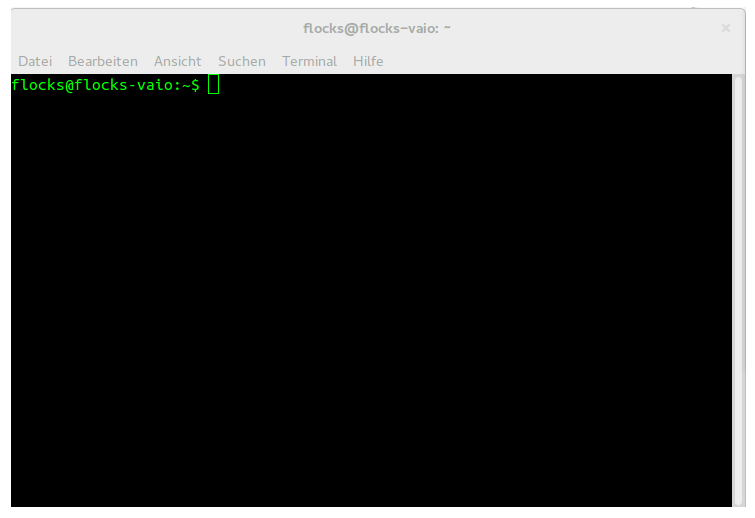
\includegraphics[width=.7\textwidth] {Bilder/bild.png}
	\caption{Screenshot}\label{MeinBild}
\end{figure}
\FloatBarrier
\blindtext
\section{Zweiter Abschnitt}
\setlength\extrarowheight{5pt}
\begin{table}[h]
	\begin{center}
	\begin{tabular}{ l l p{.5\textwidth} }
		\hline
		\emph{Model} & \textbf{RezeptZutaten.java} & Ein Softwaremodell für die Zutaten des anzuzeigenden Rezeptes. Die Datei stellt Methoden und Funktionen bereit, mit der nötige Zutaten für dieses Rezept wiedergegeben werden können. Dies kann von einer beliebigen Quelle sein. Beispielsweise über eine Schnittstelle zu einer Datenbank.\\[.2cm]
		\emph{View} & \textbf{RezeptView.jsp} & Die Werte, die aus dem Model übergeben werden, zeigt die RezeptView.jsp auf der Oberfläche an. Sie ist für das Präsentieren der Daten für den Benutzer zuständig. In diesen Dateien kann Logik enthalten sein, sollte aber nicht.\\[.2cm]
		\emph{Controller} & \textbf{RezeptAction.java} & Diese Datei ist die Verbindung zwischen der View und dem Model. Es wird entschieden, welche Aktion des Nutzers welche Reaktion zur Folge hat und die definierte View ausgewählt. Des Weiteren leitet sie die Daten aus dem Model an diese weiter. \\[.2cm]
		\hline
	\end{tabular}\caption{Beispieltabelle mit Zitat (vgl. \cite[S.~21]{struts})}
\end{center}
\end{table}
\FloatBarrier

% Verzeichnisse
\newpage
\pagestyle{empty}
\listoffigures
\listoftables
\lstlistoflistings

% Literatur
\newpage
\bibliographystyle{alphadin}
\bibliography{meinebib}

% Nach dem Inhalt
\pagestyle{plain}
\clearpage
\appendix
\pagenumbering{Roman}
\backmatter

\begin{appendices}
	\renewcommand{\thechapter}{\alph{chapter}}
	\renewcommand{\thesection}{\Alph{section}}
	\chapter{Anhang}
	\section{Quellcode}
	\subsection{Quellcode aus Datei}
		\lstinputlisting[firstline=1,lastline=23 ]{Quellcode/Example.java}
\end{appendices}

\section*{Erklärung}

Hiermit versichere ich, dass ich die vorliegende Arbeit selbständig verfasst und keine anderen als die angegebenen Quellen und Hilfsmittel benutzt habe. Ich versichere, dass ich alle wörtlich oder sinngemäß aus anderen Werken übernommenen Aussagen als solche gekennzeichnet habe, und dass die eingereichte Arbeit weder vollständig noch in wesentlichen Teilen Gegenstand eines anderen Prüfungsverfahrens gewesen ist.

\vspace*{3em}

\newcommand*{\SignatureAndDate}[1]{
	\par\noindent\makebox[52mm]{\hrulefill}     \hfill\makebox[65mm]{\hrulefill}
	\par\noindent\makebox[52mm][l]{Ort, Datum}	\hfill\makebox[62mm][l]{#1}
}

\SignatureAndDate{Unterschrift}


\end{document}